\section{
  Dusty vertical shear instability}\label{results} 

%When $\tstop=0$ we may construct exact dusty equilibra by specifying
%the dust-to-gas ratio, as described in \S\ref{eqm}. 


We present numerical solutions to the linearized
equations to examine the effect of dust on the VSI. 
We consider perfectly coupled dust ($\tstop=0$) so that the 
equilibria defined in \S\ref{eqm} are exact steady states. 

For simplicity, we mostly consider constant midplane
dust-to-gas ratios $\epsilon_0$ and its characteristic height
$H_\epsilon$. The latter is specified via the dust layer thickness
$\Hd(r_0)$. (We will allow for radial dependices in $\epsilon_0$ and
$H_\epsilon$ in \S\ref{varHd}.)   
These, together with the perturbation wavenumber $k$, comprises main the
parameters of the linear problem. We fix the radial power-law index
for the midplane gas density to $p = -1.5$, that for the
temperature profile to $q=-1$; and set the gas disk aspect-ratio
$h_\mathrm{g}=0.05$. These are fiducial values used by 
\citet[][\citetalias{lin15} in this section]{lin15}. 

Two boundary conditions are needed for the $\tstop=0$
problem. This is expected since this problem is equivalent to
adiabatic hydrodynamics \citep[e.g.][]{lubow93}. We 
impose solid boundaries so that $\delta v_z(\pm\zmax)=0$.  
We solve the linearized equations as a generalized eigenvalue problem 
using a pseudo-spectral code adapted from \cite{lin15}. Amplitudes 
are expanded in Chebyshev polynomials up to order $N_z=512$. We check
results using Eq. \ref{vsi_check}.    

\subsection{Qualitative expectations}\label{vsi_est}
\cite{lin15} found the appropriate way to compare 
destabilizing vertical shear to stabilizing vertical buoyancy is
$r\p_z\Omega/\OmK$ against $N_z^2/\OmK^2$. We see from \S\ref{vertshear}
and \S\ref{vbuoyancy} that $|r\p_z\Omega|\sim q h_\mathrm{g}\OmK$ for a
thin, gas dominated disk; while $N_z^2\sim \epsilon\OmK^2$. Thus we
expect dust-induced buoyancy forces to stabilize the disk against the
VSI where $\epsilon \gtrsim h_\mathrm{g}$. 

%\begin{align}

\subsection{Effect of dust-loading}
We first vary the midplane dust-to-gas ratio 
$\epsilon_0\in[10^{-3},1]$, fixing the dust thickness to  
$\Hd=0.99\Hg$. Then  $\epsilon$ is roughly constant with height. We
set the vertical domain to $\zmax=5\Hg$.  

Fig. \ref{compare_vshear_fixHd} compares the basic state
vertical shear rate, which is destabilizing, and the vertical buoyancy
frequency, which is stabilizing. For the nearly dust-free disk
$\epsilon_0=10^{-3}$ the vertical shear dominates buoyancy for all
$|z|>0$. However, a heavy dust-load with $\epsilon_0=1$ renders the 
buoyancy to dominate over vertical shear in the disk atmosphere 
$|z|\gtrsim 2.5$. We thus expect instability all heights for 
$\epsilon_0=10^{-3}$, but to be restricted to the midplane for
$\epsilon_0=1$. 

\begin{figure}
  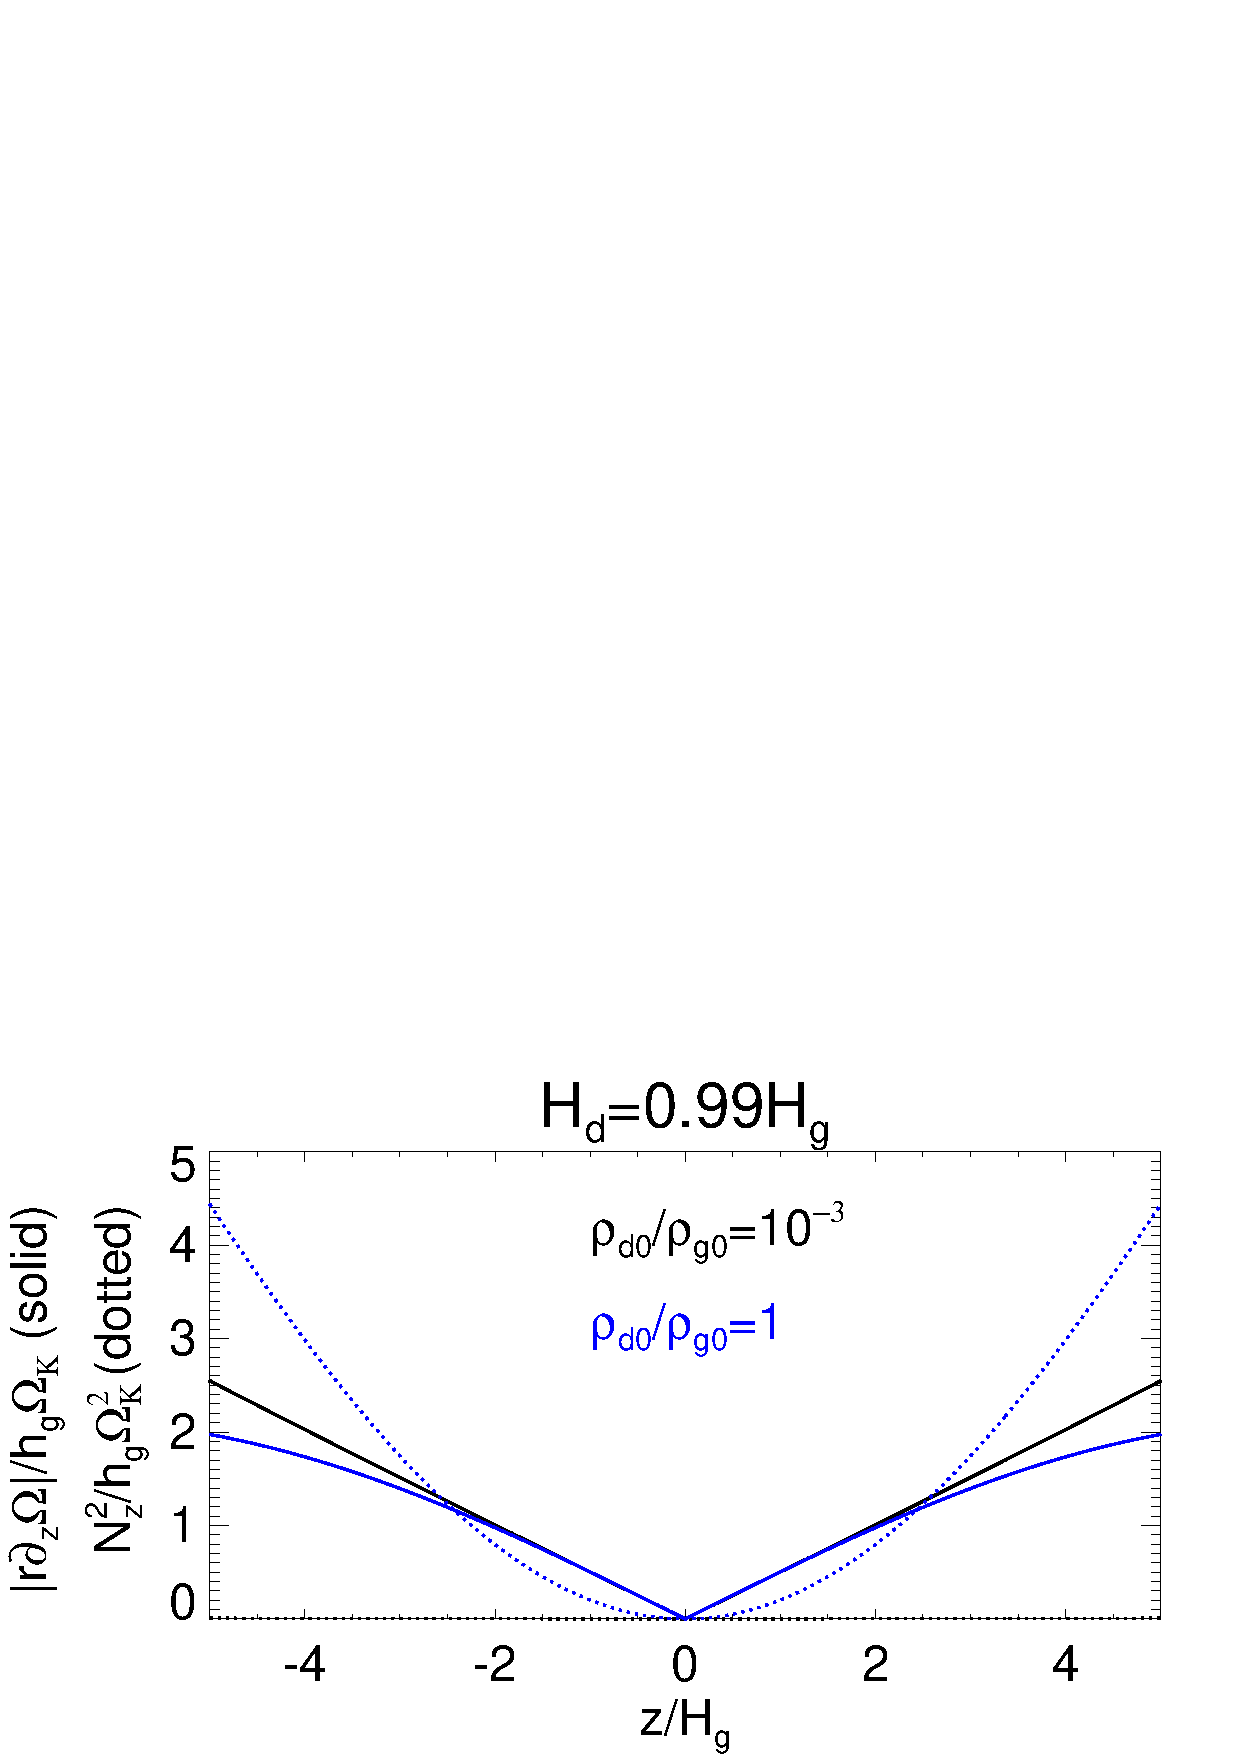
\includegraphics[width=\linewidth]{figures/compare_vshear_Nz2_fixHd} 
  \caption{Vertical shear rate (solid) compared to vertical buoyancy
    (dotted) in a locally isothermal, dusty disl with midplane dust-to-gas ratio
    of $\epsilon_0=10^{-3}$ (black) and $\epsilon_0=1$ (blue). 
    The dust layer thickness is fixed to $\Hd=0.99\Hg$ so the 
    dust-to-gas ratio $\epsilon$ is approximately constant with
    height. 
    \label{compare_vshear_fixHd}
    }
\end{figure}

Fig. \ref{vsi_dust_loading} show unstable modes for different values
of $\epsilon_0$ with fixed perturbation wavenumber  $k\Hg = 30$. The
eigenvalue distributions for $\epsilon_0 \leq 10^{-2}$ are similar to the
dust-free fiducial case considered by \citetalias{lin15}. This is
expected since $\epsilon_0 < \hgas$ (\S\ref{vsi_est}). Eigenvalues 
consists 
of the roughly horizontal `body modes' and the nearly-vertical
`surface modes'. The latter is due to the imposed vertical boundaries
\citep{barker15}.  

We find that increasing the dust-to-gas ratio reduce VSI growth
rates. Notably, `surface modes', which are typically fastest growing in
the dust-free case, are surpressed in dusty disks for $\epsilon_0\geq
0.1$ (i.e. $\epsilon_0> \hgas$).  
The body modes' growth rates remain $ O(h_\mathrm{g}\OmK)$ 
but their oscillation frequency increases with
$\epsilon_0$. %i.e. increases with buoyancing freq 
The total number of modes do not change
significantly. This is in contrast with the effect of increasing
cooling times, where \citetalias{lin15} find fewer unstable modes.
%until the system is eventually completely stable. 

\begin{figure}
  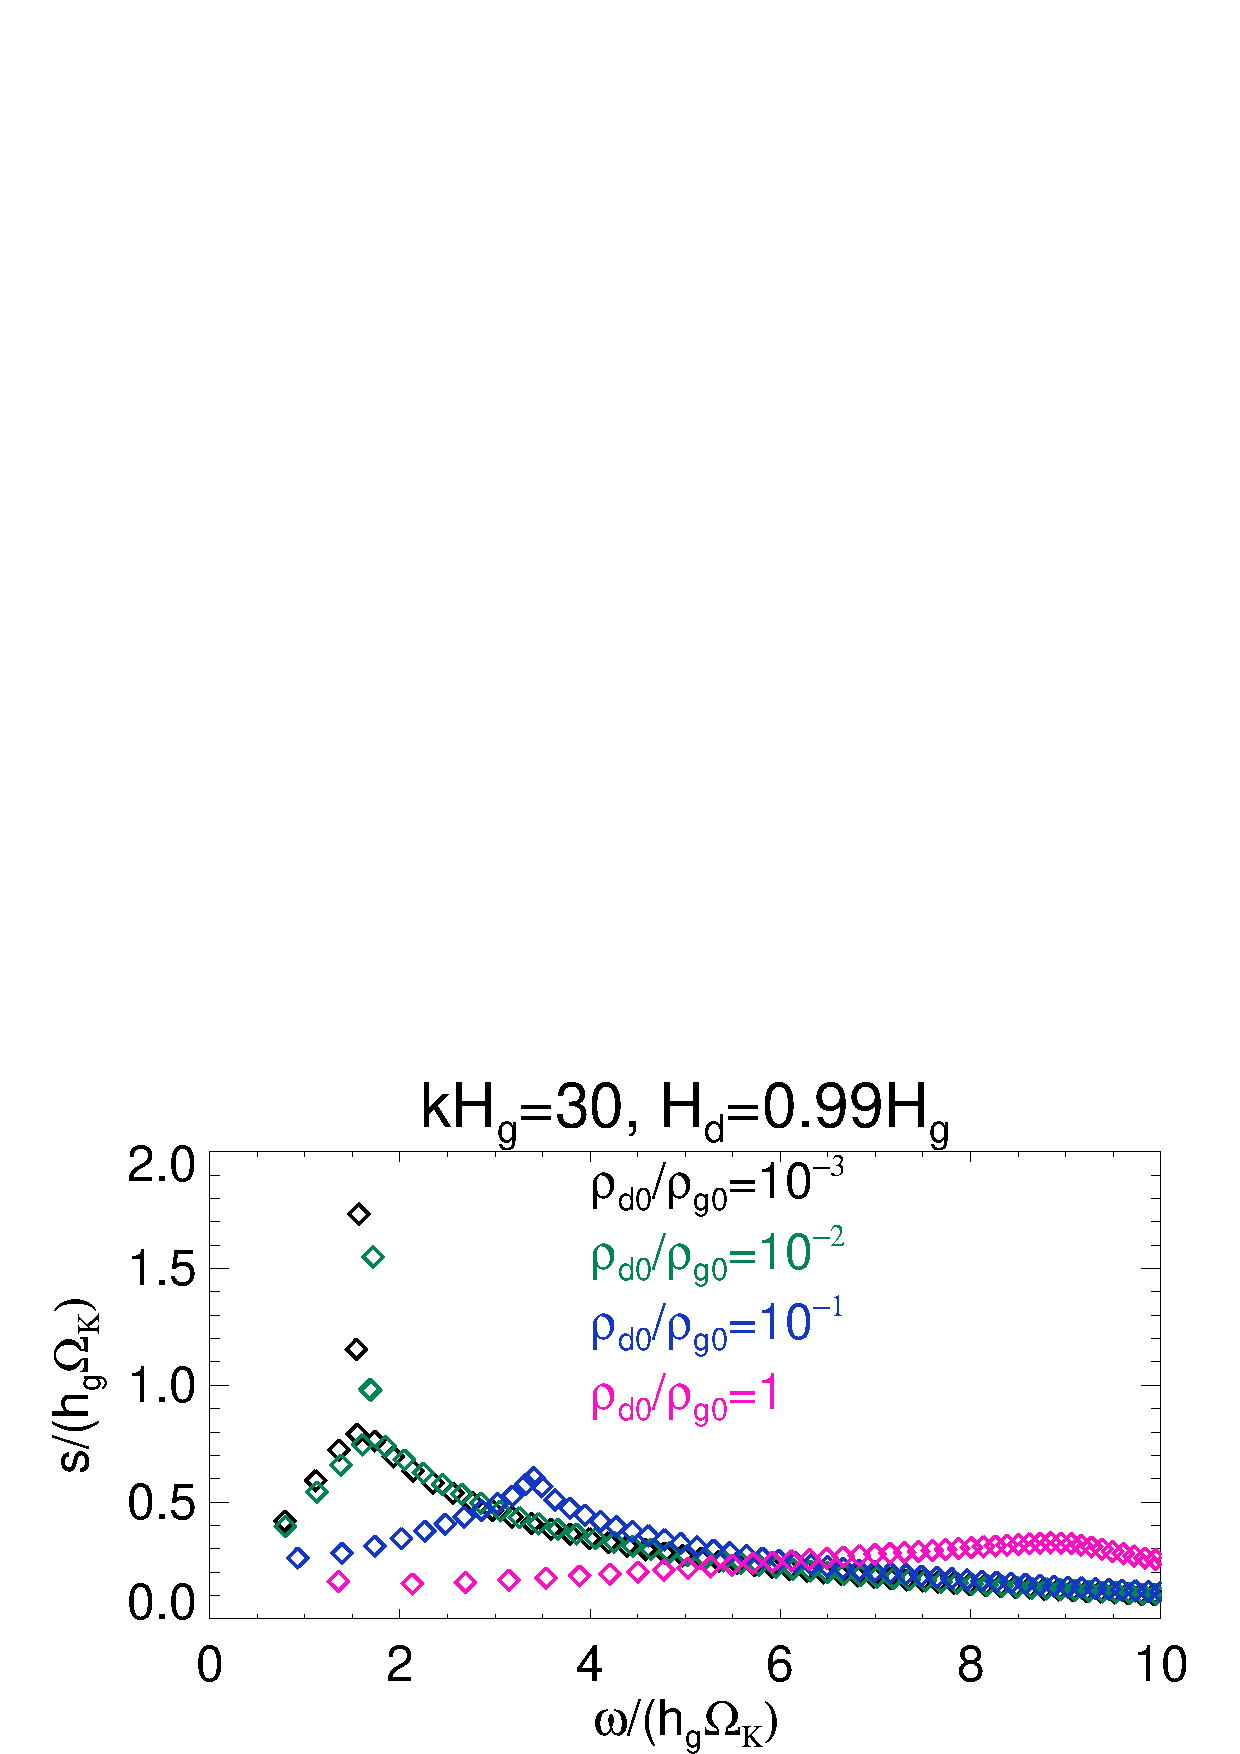
\includegraphics[width=\linewidth]{figures/compare_eigenvals_kx30Hd1} 
  \caption{Unstable modes in a locally isothermal, perfectly coupled
    dusty disk with fiducial parameters
    $(p,q,h_\mathrm{g}, \Hd/\Hg )=(-1.5,-1,0.05, 0.99)$. The real
    frequency $\omega$ and growth rates $s$ are shown for a range of
    midplane dust-to-gas ratios $\epsilon_0=\rho_\mathrm{g0}/\rho_\mathrm{d0}$. 
    \label{vsi_dust_loading}
    }
\end{figure}

The lowest frequency `fundamental' body mode is energetically dominant
because the entire disk column is perturbed \citep[cf. surface modes
  which only disturb the disk boundaries,][]{umurhan16c}. In Fig. \ref{vsi_dust_loading2d}
we compare the fundamental mode between the nearly 
dust-free case $\epsilon_0=10^{-3}$ an a dusty disk with
$\epsilon_0=1$. Dust-loading preferentially
stabilizes the disk atmosphere against the VSI, restricting
meridional motions to $|z|\lesssim 2\Hg$. 
This is consistent with Fig. \ref{compare_vshear_fixHd} comparing the basic state vertical
shear and buoyancy. Notice also the perturbed dust-to-gas ratio,
$\delta\epsilon$, shifts from being maximized at the disk boundaries
to the midplane.  

\begin{figure}
%  \includegraphics[scale=0.54, clip=true, trim=0cm 2.5cm 0cm 0cm]{figures/result2d_dg1d-3.ps}\\
%  \includegraphics[scale=0.54]{figures/result2d_dg1.ps} 
\includegraphics[scale=0.32, clip=true, trim=0.5cm 0cm 3cm 0cm]{figures/result2d_dg1d-3.ps}\includegraphics[scale=0.32, clip=true, trim=1.8cm 0cm 0cm 0cm]{figures/result2d_dg1.ps}
  \caption{Fundamental dusty VSI mode in real space for midplane dust-to-gas
    ratio $\epsilon_0=10^{-3}$ (left) and $\epsilon_0=1$
    (right). The color scale shows the perturbation to the
    dust-to-gas ratio, $\delta\epsilon$; and the arrows show
    $\sqrt{\rho}\left(\dd v_x, \dd v_z\right)$. 
    \label{vsi_dust_loading2d}
    }
\end{figure}

In Fig. \ref{vsi_dust_loading_vareps} we plot the growth rates as a
function of $\epsilon_0$ for different perturbation wavenumbers $k$. We
find that dust-loading stabilizes the VSI more effectively for shorter
wavelength perturbations. This is because for high wavenumbers the
dominant modes are surface modes, which are effectively stabilized by
dust-loading since bouyancy forces are larges near the disk
boundaries. The figure suggest that VSI becomes much less efficient
for $\epsilon_0\gtrsim 0.1$ and $k\Hg\gtrsim 50$. 

\begin{figure}
  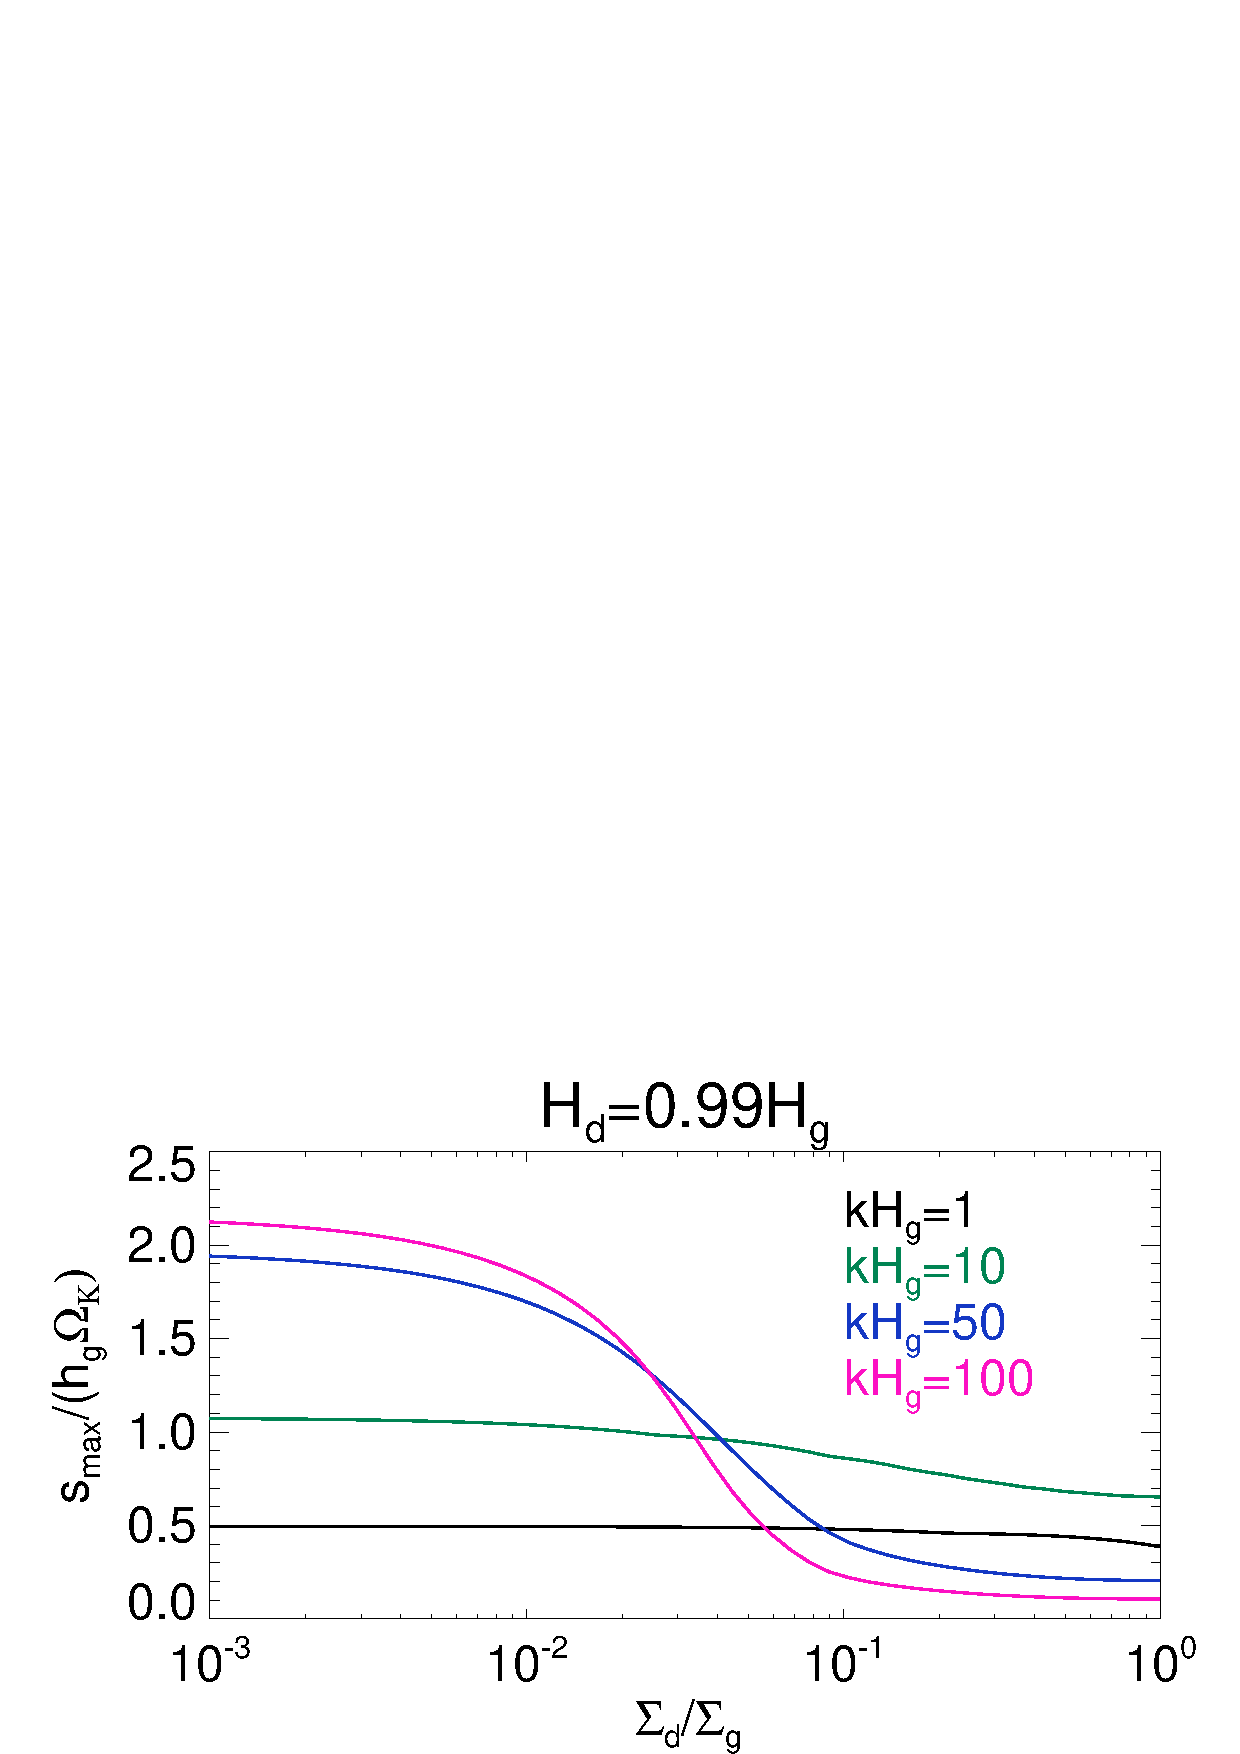
\includegraphics[width=\linewidth]{figures/compare_eigenvals_vareps2} 
  \caption{Maximum growth rate of the dusty VSI as a function of the
    midplane dust-to-gas ratio $\epsilon_0$ for perturbations with
    different radial wavenumbers $k$. The dust layer thickness is
    fixed to $\Hd\simeq \Hg$. 
    \label{vsi_dust_loading_vareps}
    }
\end{figure}




\subsection{Effect of dust thickness} 
We now vary the dust layer thickness $\Hd$ but fix the metalicity 
$Z \equiv \epsilon_0 \Hd/\Hg = 0.03$. This then gives the
required midplane dust-to-gas ratio. Since we will consider thin dust
layers, here we use a smaller 
domain with $\zmax=2\Hg$ so that $\epsilon$ does not become
too small. 

We analyze two disks with $\Hd=0.1\Hg$ and 
$\Hd=0.99\Hg$. Fig. \ref{compare_vshear_fixZ} compares the vertical
vhear rate and buoyancy frequency. For $|z|\gtrsim 0.4\Hg$ the two
disks have the same profile with vertical shear dominating over
buoyancy. We thus expect perturbations away from the disk midplane in 
both cases. For $|z|\lesssim 0.4\Hg$, a thin dust 
layer with $\Hd=0.1\Hg$ boosts the vertical shear rate, but the
associated buoyancy is larger still, implying the mid-plane should be
stable. 
%Thus we expect the mid-plane of 
%the disk with $\Hd=0.1\Hg$ to have limited vertical motions.  

\begin{figure}
  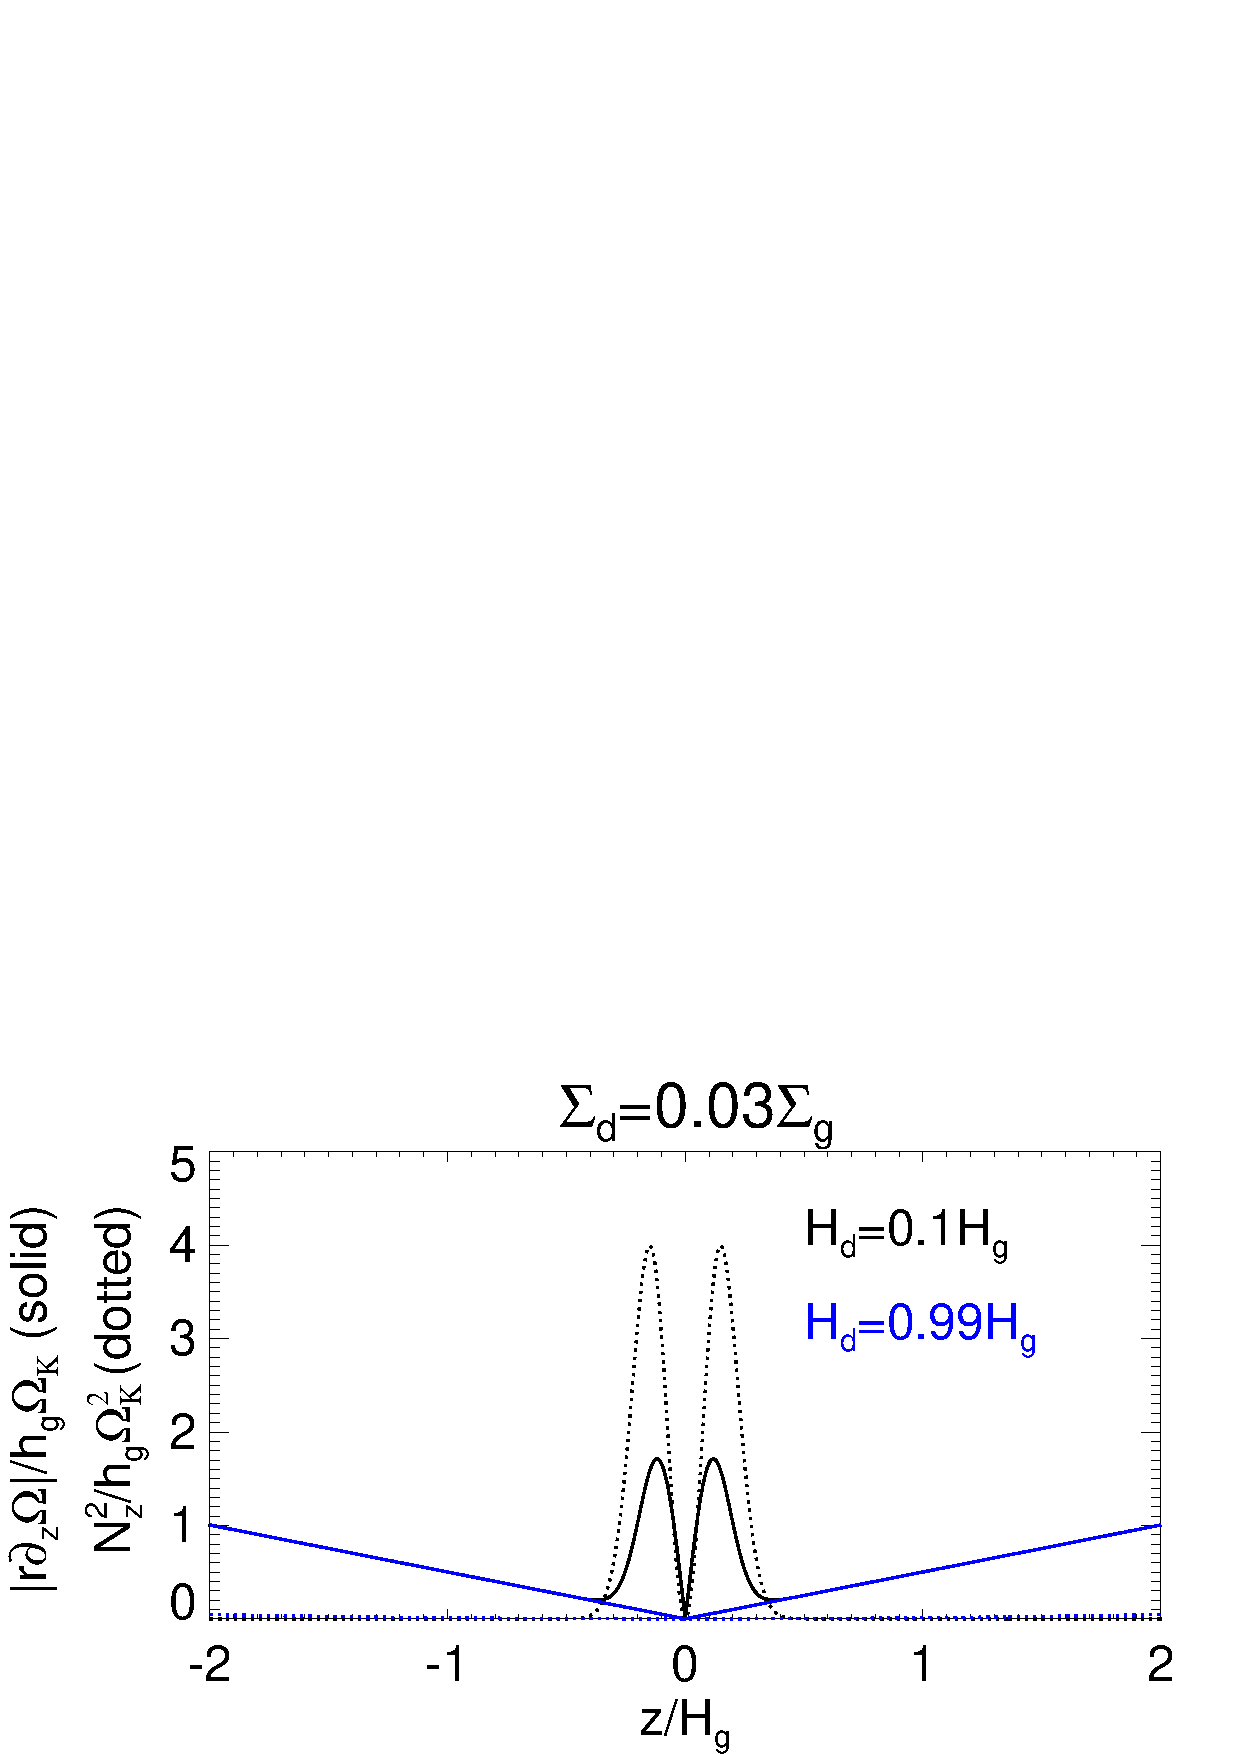
\includegraphics[width=\linewidth]{figures/compare_vshear_Nz2_fixZ} 
  \caption{Vertical shear rate (solid) compared to vertical buoyancy
    (dotted) in a locally isothermal, dusty disk 
    with metalicity $Z=0.03$ and dust thickness $\Hd=0.1\Hg$
    (black) and $\Hd=0.99\Hg$ (blue). 
    \label{compare_vshear_fixZ}
    }
\end{figure}

Fig. \ref{result2d_fixZ} compares the fastest growing VSI body modes  
with $k\Hg=30$ for the two cases above.\citepalias[The thinner domain
  adopted here eliminates surface modes, ][]{lin15}.   
We find very similar mode 
frequencies 
\begin{align*}
  \sigma = \begin{cases}
    \left(0.3053\ii - 0.8142\right)h_\mathrm{g}\OmK & \Hd=0.99\Hg, \\
    \left(0.3178\ii - 1.2237\right)h_\mathrm{g}\OmK & \Hd=0.1\Hg,
  \end{cases}
\end{align*}
since the vertical shear profile is similar throughout most of the
disk. However, meridional motions are surpressed near the midplane of
the $\Hd=0.1\Hg$ disk, as expected from the larger buoyancy frequency
as compared to vertical shear there. This leads to a structure
analogous to PPD dead zones: a quiescent midplane between active
surface layers \citep{gammie96}.  


\begin{figure}
  \includegraphics[scale=0.32, clip=true, trim=0.5cm 0cm 3cm 0cm]{figures/result2d_Hd1.ps}\includegraphics[scale=0.32, clip=true, trim=1.8cm 0cm 0cm 0cm]{figures/result2d_Hd0d1.ps} 
  \caption{Fastest-growing dusty VSI mode in real space for midplane
    dust layer thickness $\Hd=0.99\Hg$ (left) and $\Hd=0.1\Hg$
    (right). The dust content is fixed to
    $\Sigma_\mathrm{d}=0.03\Sigma_\mathrm{g}$. 
    The color scale shows the perturbation to the
    dust-to-gas ratio, $\delta\epsilon$; and the arrows show
    $\sqrt{\rho}\left(\dd v_x, \dd v_z\right)$.
    \label{result2d_fixZ}
    }
\end{figure}

Fig. \ref{compare_eigenvals_fixZ} shows the maximum VSI growth rates
as a function of $\Hd$. As before, we find growth
rates are most affected by the vertical structure of the dust layer
when the perturbation wavenumer is large. Notice VSI growth rates converge as
$\Hd\to 0$. %to dust free values?    
Thus a thin dust layer, however large its associated vertical shear,
does not affect the VSI. The non-monotonic behavior for $\Hd\gtrsim
0.5\Hg$ arises because the vertical buoyancy frequency 
\begin{align*}
N_z^2(H_d;z,Z) \simeq &Z\Hg z^2
\exp{\left(-\frac{z^2}{2\Hg^2}\right)}\OmK^2\notag\\
&\times 
\frac{1}{\Hd}\left(\frac{1}{\Hd^2} -
\frac{1}{\Hg^2}\right)\exp{\left(-\frac{z^2}{2\Hd^2}\right)}  
\end{align*}
is a non-monotonic function of $\Hd$ at fixed $z$. At $z=\Hg$ and $z=2\Hg$
the buoyancy frequency is maximized for $\Hd\simeq0.5\Hg$ and
$\Hd\simeq 0.8\Hg$, respectively. This is consistent with the abscissa
of minima in growth rates in Fig. \ref{compare_eigenvals_fixZ}. 

\begin{figure}
  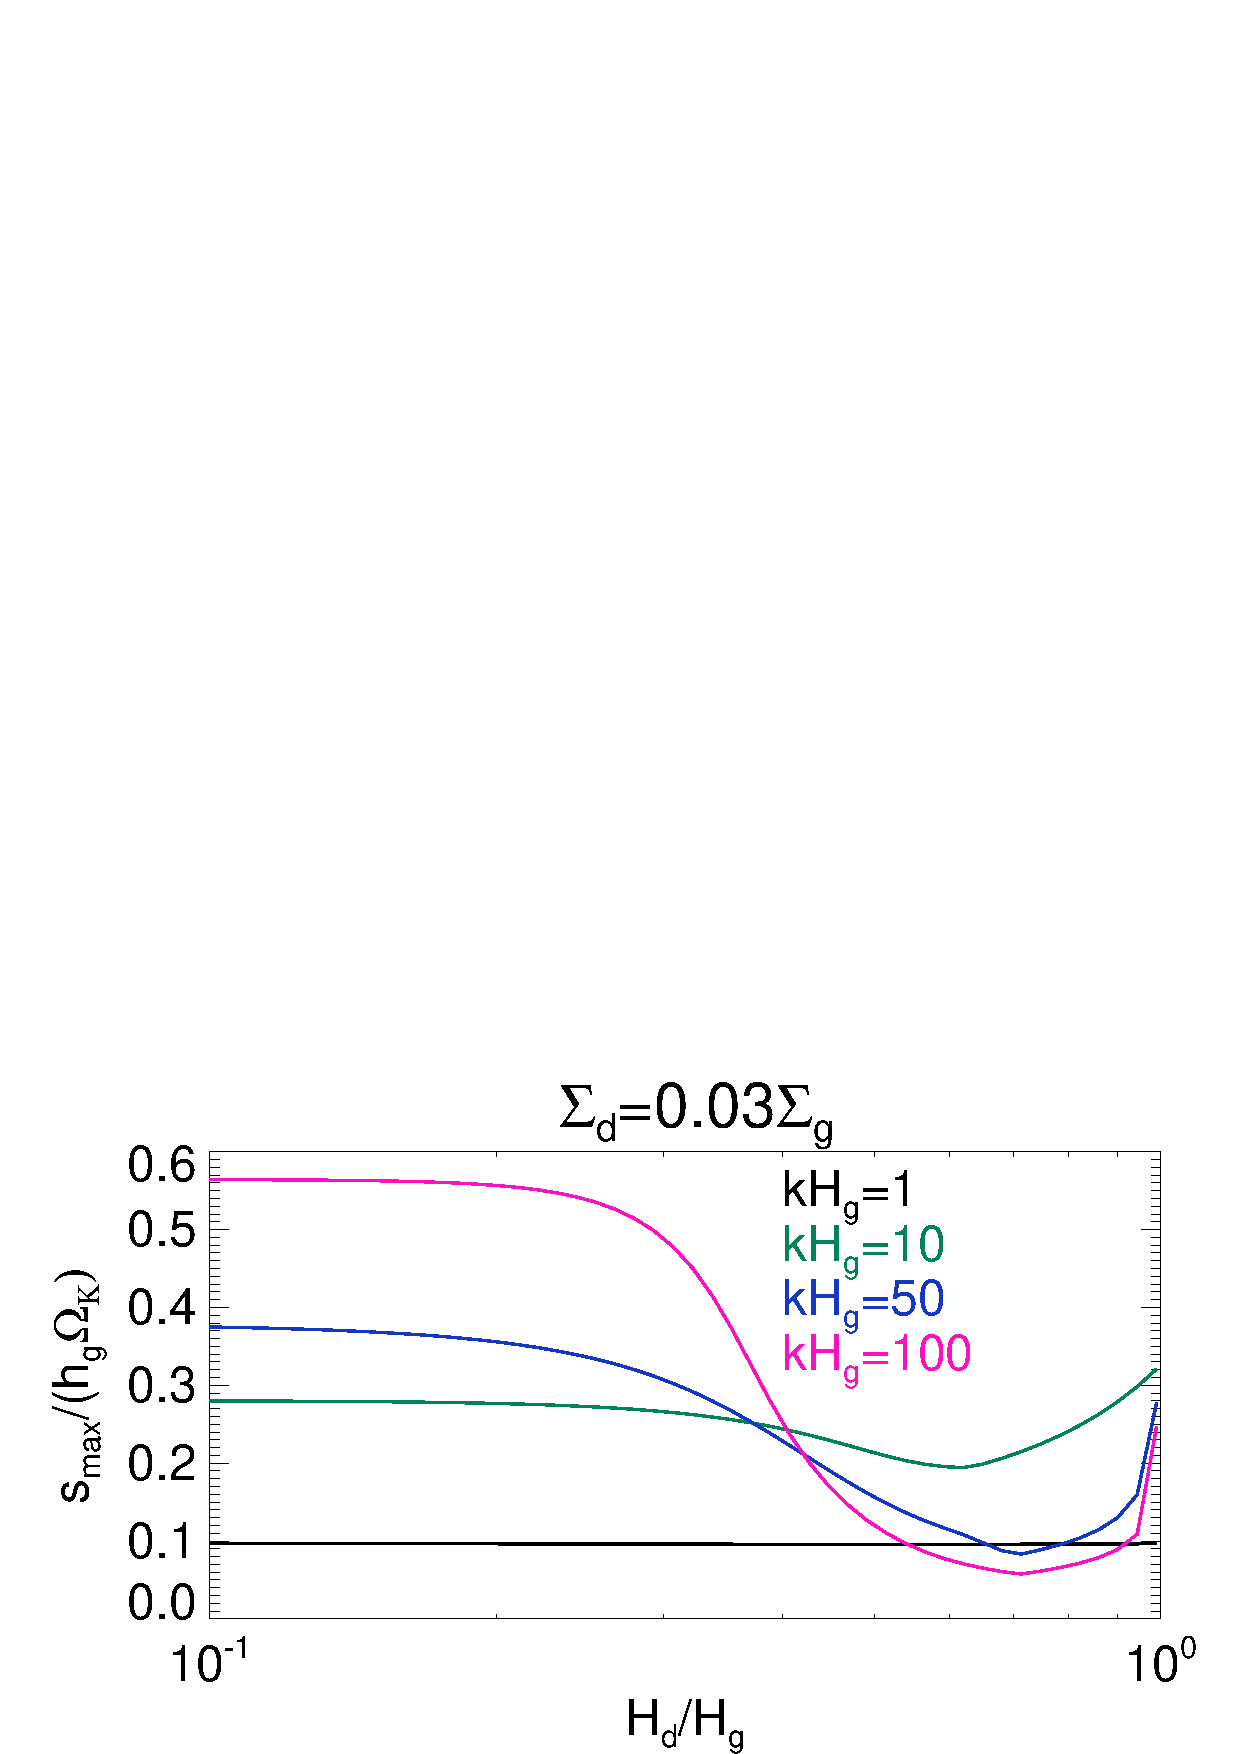
\includegraphics[width=\linewidth]{figures/compare_eigenvals_fixZ} 
  \caption{Maximum VSI growth rate for different perturbation
    wavenumbers $k$ as a function of the dust layer
    thickness $\Hd$ at fixed metalicity $Z=0.03$. 
    \label{compare_eigenvals_fixZ}
    }
\end{figure}


\subsection{Effect of a radially-varying dust-to-gas ratio}\label{varHd}
{\bf move to appendix?}

Here we allow the dust-to-gas ratio $\epsilon$ to depend on
$r$. Specifically we let $\epsilon_0\propto r^{-1}$ and
$H_\epsilon \propto \Hg$ (cf. constant values in the previous
calculations). Then
\begin{align*}
  \frac{\p\epsilon}{\p r} =
  \left(\frac{z^2}{H_\epsilon^2}\frac{d\ln{\Hg}}{dr} -
    \frac{1}{r}\right)\epsilon.   
\end{align*}
We fix $Z=0.01$, $\Hd=0.8\Hg$ at $r=r_0$, and
$k\Hg=30$.      

Fig. \ref{compare_vshear_varHd} shows that a radially-varying
dust-to-gas ratio increases the magnitude of the vertical shear rate
away from the midplane (see also Eq. \ref{vshear2}). Thus we find
higher VSI growth rates, as shown in Fig. \ref{vsi_dust_varHd}. 
Surfaces modes are more effectively enhanced by the additional vertical 
shear induced by $\p_r\epsilon$. However, all growth rates remain
$O(\hgas\OmK)$. Importantly, the increase in the growth rate of the
fundamental mode is small. Thus we do not expect the radial
dependence in $\epsilon$ to significantly affect the VSI in a dusty
disk. 

\begin{figure}
  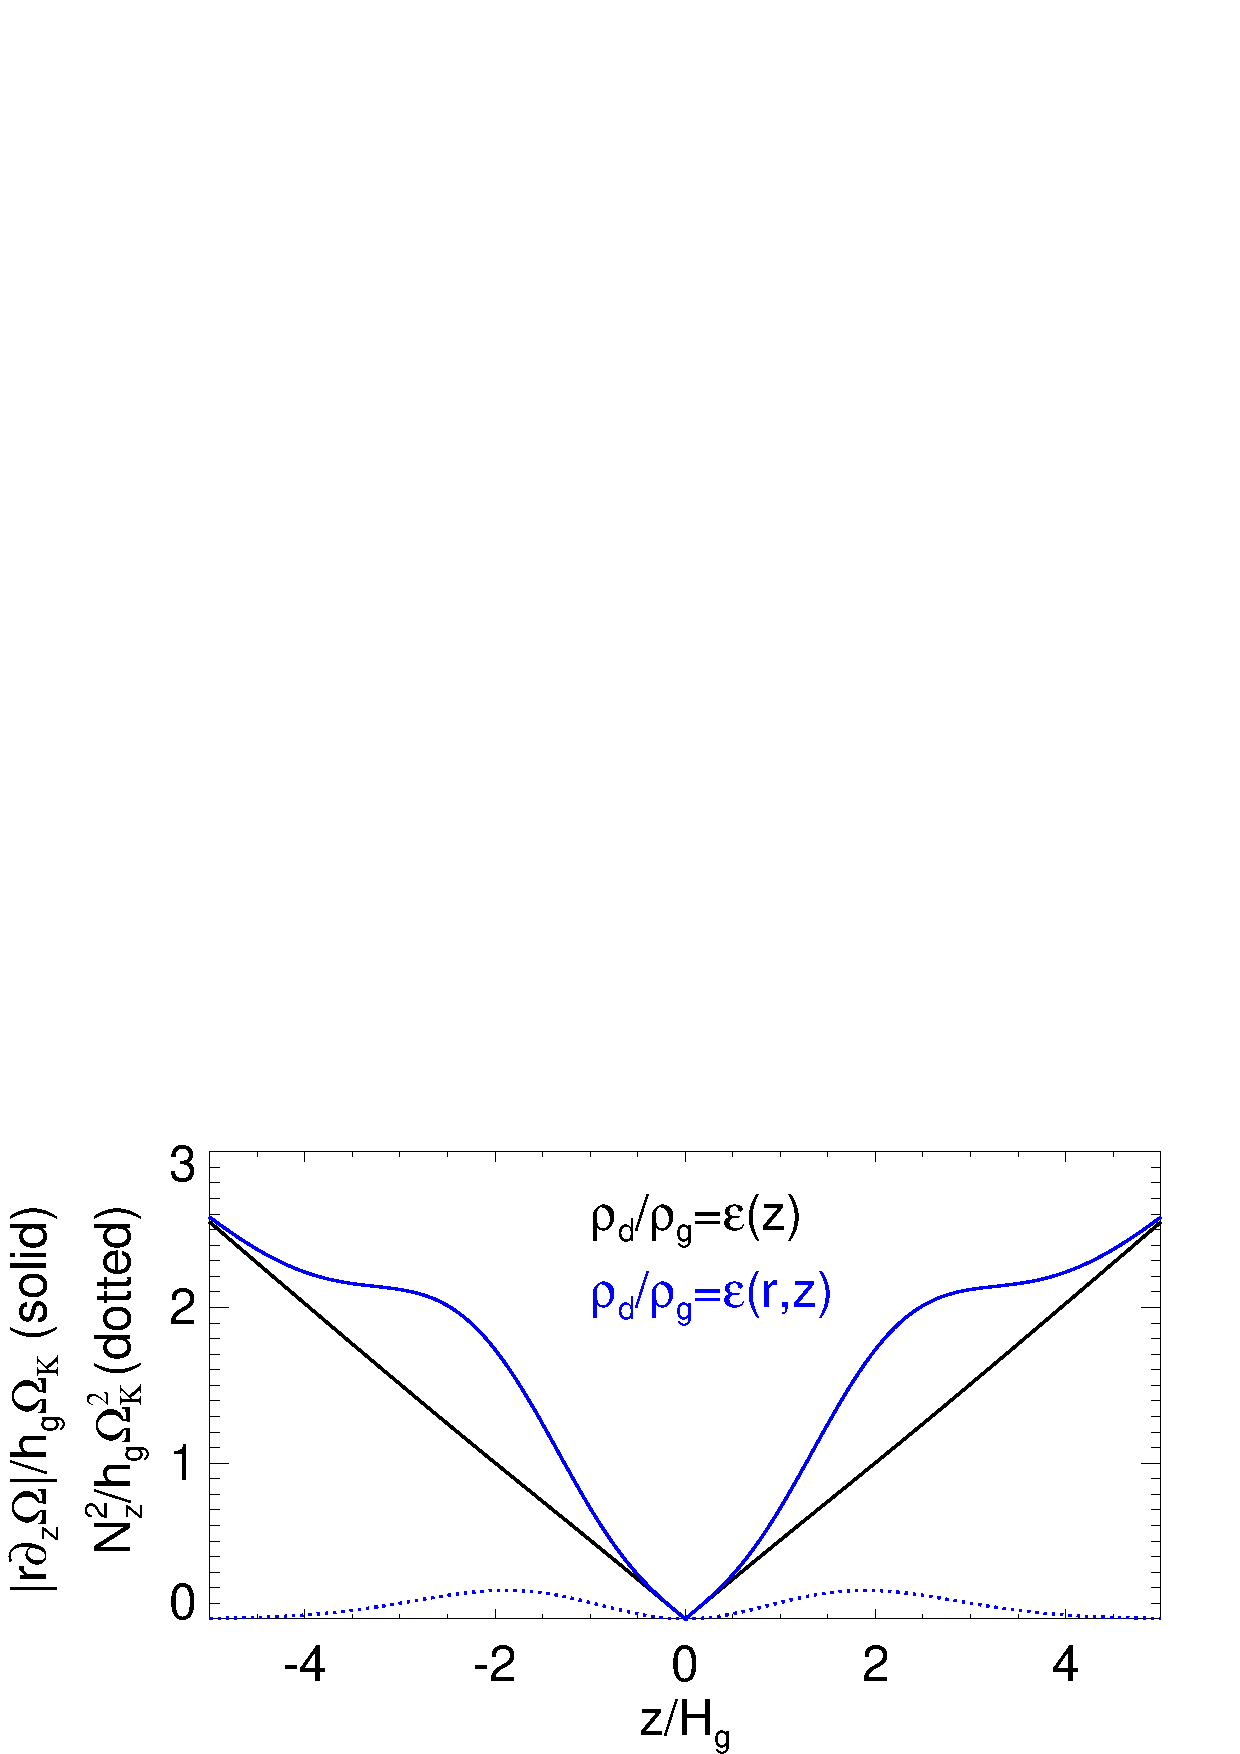
\includegraphics[width=\linewidth]{figures/compare_vshear_Nz2_varHd} 
  \caption{Vertical shear rate (solid) compared to vertical buoyancy
    (dotted) in a locally isothermal, dusty disk 
    with metalicity $Z=0.01$ and dust thickness $\Hd=0.8\Hg$.
    Black curves assume a dust-to-gas ratio that only depends on
    height; whereas the blue curve also allows a radial dependence in
    $\epsilon$. See text for details.  
    \label{compare_vshear_varHd}
    }
\end{figure}



\begin{figure}
  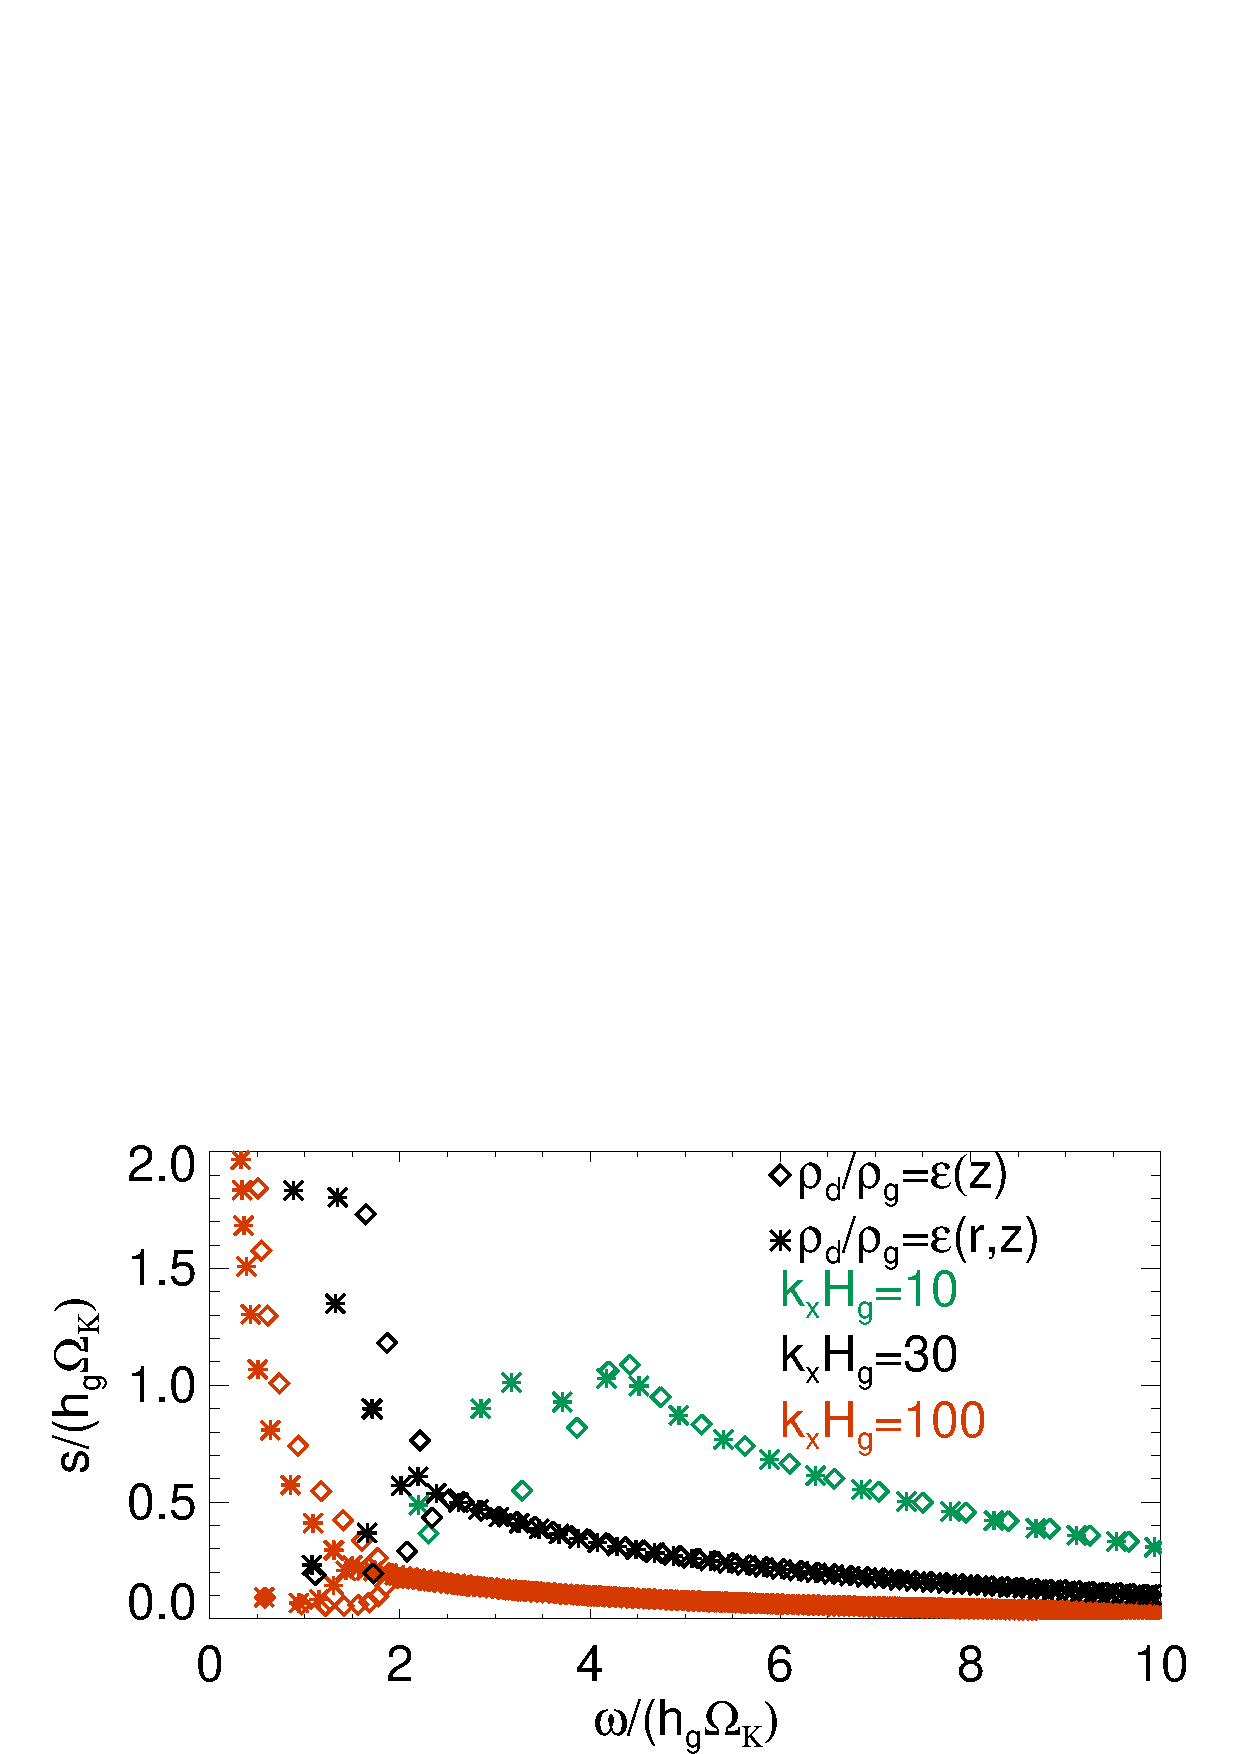
\includegraphics[width=\linewidth]{figures/compare_eigenvals_varHd} 
  \caption{Unstable VSI modes in the disk models of
    Fig. \protect\ref{compare_vshear_varHd}.  
    \label{vsi_dust_varHd}
    }
\end{figure}



\subsection{Validity}
We considered $\tstop=0$ in order to perform stability analysis on an
exact steady state. When $\tstop\neq0$, a 
disk initialized as in \S\ref{eqm} will evolve 
due to dust-gas relative drift. In particular, in the
absence of turbulent/diffusive processes, dust particles settle to the
midplane on a timescale $t_\mathrm{settle}\sim 1/\tstop\OmK^2$
\citep{takeuchi02}. However, we expect the above results to remain
valid provided the VSI growth
timescale $t_\mathrm{grow}\ll t_\mathrm{settle}$. Since 
VSI growth rates are $O(h_\mathrm{g}\OmK)$, we require 
\begin{align}
  \tstop\OmK \ll h_\mathrm{g}. 
\end{align} 
For thin PPDs with $h_\mathrm{g}\sim 0.05$, this is satisfied 
for $\tstop\OmK \ll O(10^{-2})$.  
